\documentclass{beamer}
\usepackage[english]{babel}
\setbeamertemplate{navigation symbols}{}
\setbeamertemplate{frametitle}[default][center]
\setbeamertemplate{bibliography item}{\insertbiblabel}
\usefonttheme[onlymath]{serif}

\usepackage{graphicx}
\graphicspath{ {./images/} }
\usepackage{amsmath}
\usepackage{wrapfig}

\title{Research Presentation}
\subtitle{COMP230}
\author{1706966}

\begin{document}

\begin{frame}
	\maketitle
\end{frame}

\begin{frame}{Background}
	Depression is a common illness worldwide, with more than 300 million people affected. When long-lasting and with moderate or severe intensity depression may become a serious health condition. At its worst, depression can lead to suicide. Close to 800 000 people die due to suicide every year. Suicide is the second leading cause of death in 15-29 year-olds\cite{DepressionStats}.
\end{frame}

\begin{frame}{The Issue}
	During this preliminary research it has been confirmed that there are no guidelines specific to the video game industry in regards to how suicide and depression are handled in video games.\vspace{5mm} %5mm vertical space
	
	Popularised guidelines do exist for portraying suicide in the news\cite{world2017preventing}\cite{nepon2009media} and drama adaptations\cite{DramaGuidelines}. \vspace{5mm} %5mm vertical space
	
	The drama adaptation guidelines match best with a video game environment and could possibly be implemented as guidelines for video games. However due to the artistic style, interactivity and immersion of video games it might be best to form more specific industry guidelines.   
\end{frame}

\begin{frame}{Importance}
	\begin{wrapfigure}{L}{0.5\textwidth} %this figure will be at the right
		\centering
		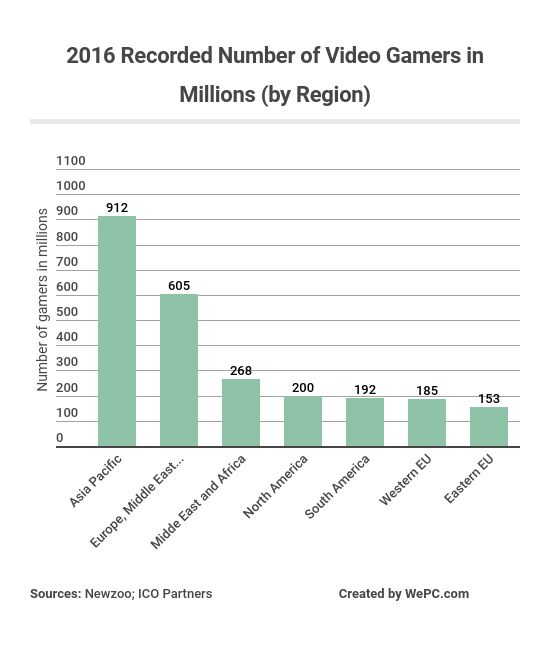
\includegraphics[width=0.5\textwidth]{numberOfGamers}
	\end{wrapfigure}
	With over 2.5 billion people playing video games the ability for games to effect players is dramatic. 
\end{frame}

\begin{frame}{National Statistics}
		\begin{itemize}
		\item 6,213 suicides in the UK and Ireland last year\cite{death2018suicide}.
		\item In the UK men are three times as likely to take their own lives than women, and in the Republic of Ireland four times as likely\cite{death2018suicide}.
		\item 19.7\% of over 16's in the UK showed symptoms of anxiety or depression in 2014\cite{MentalStatistics}.
		\item A higher proportion of women (22.5\%) than men (16.8\%) indicated they had some feelings of depression\cite{MentalStatistics}.
	\end{itemize}
\end{frame}
\begin{frame}{References}
	\bibliographystyle{ieeetran}
	\bibliography{references}
\end{frame}
\end{document}